
\documentclass[11pt]{article}


\usepackage[pdftex]{graphicx}
\usepackage{url} 
\usepackage[dvips, bookmarks, colorlinks=false, pdfborder={0 0 0}, pdftitle={<pdf title here>}, pdfauthor={<author's name here>}, pdfsubject={<subject here>}, pdfkeywords={<keywords here>}]{hyperref} 
\usepackage[final]{pdfpages}
\usepackage{multirow}


\title{XSM \\ eXperimental String Machine \\
Version 1.0}
\author{Dr. K. Muralikrishnan  \\ \texttt{kmurali@nitc.ac.in} \\ {NIT Calicut} }


\begin{document}

\maketitle
\pagebreak

%......................Table of Contents............................%
\thispagestyle{plain}

\tableofcontents
\pagebreak


\section{Introduction}

\subsection{Brief Machine Description}
The machine simulator is known as Experimental String Machine (XSM). It is an interrupt driven uniprocessor machine. The machine handles data as strings. A string is a sequence of characters terminated by '\textbackslash 0'. The length of a string is atmost 16 characters including '\textbackslash 0'. Each of these strings is stored in a \textbf{word}  (Refer Section \ref{sec:mem}). The machine interprets a single character also as a string.

\subsection{Components of the Machine}

\begin{figure}[hbtp]
\begin{center}
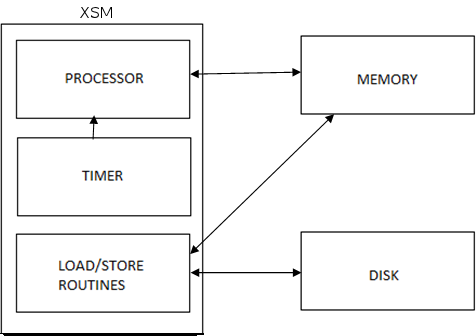
\includegraphics[scale=0.5]{block.png}
\end{center}
\caption{Components of the Machine}
\end{figure}


\begin{itemize}
\item \textbf{Disk} : It is a non-volatile storage that stores user programs (executables) and data files. The Operating System code is also stored in the disk.

\item \textbf{Memory} : It is a volatile storage that stores the programs to be run on the machine as well as the operating system that manages the various programs.
\item \textbf{Processor} : It is the main computational unit that is used to execute the instructions.
\item \textbf{Timer} : It is a device that interrupts the processor after a pre-defined specific time interval.
\item \textbf{Load/Store} : It is a macro that performs the functionalities of DMA (Direct Memory Access) controller. (Refer Section \ref{sec:inst})
\end{itemize}






\section{Registers}

\subsection{Introduction}
The XSM architecture maintains 26 registers (each one \textbf{word}).

\subsection{Register Set}
There are 16 General Purpose Registers (GPR), \texttt{R0 - R15}, of which \texttt{R0 - R7} are Program Registers and \texttt{R8 - R15} are Kernel Registers. There are 4 temporary registers \texttt{T0 - T3} which are reserved for code translation. The registers \texttt{T0 - T3} are not intended to be used by the system programmer. In addition to these 20 registers there are 6 Special Purpose Registers(SPR) namely \texttt{BP} (Base Pointer), \texttt{SP} (Stack Pointer), \texttt{PID} (Process Identifier), \texttt{IP} (Instruction Pointer), \texttt{PTBR} (Page Table Base Register) and \texttt{PTLR} (Page Table Length Register).


\begin{center}
\begin{tabular}{|c|c|}
\hline Name & Register \\ 
\hline Program Register & R0-R7 \\ 
\hline Kernel Register & R8-R15 \\ 
\hline Temporary Registers & T0-T3 \\ 
\hline Base Pointer & BP \\ 
\hline Instruction Pointer & IP \\ 
\hline Stack Pointer & SP \\ 
\hline Process Identifier & PID \\
\hline Page Table Base Register & PTBR \\
\hline Page Table Length Register & PTLR \\
\hline
\end{tabular} 
\end{center}


\section{Memory}
\label{sec:mem}

\subsection{Introduction}

%\begin{figure}[hbtp]
%\begin{center}
%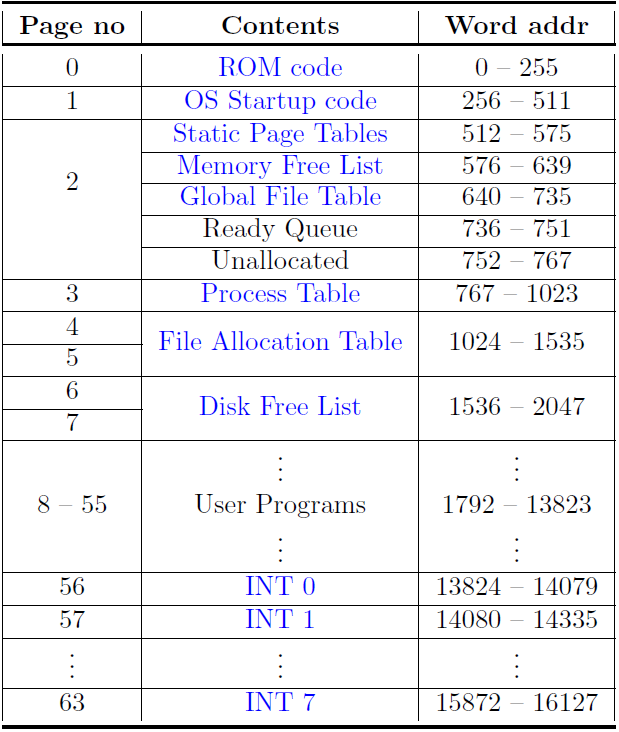
\includegraphics[scale=0.5]{memoryblockdiagram.png}
%\end{center}
%\caption{Main Memory Block Diagram}
%\end{figure}

\begin{itemize}
\item The basic unit of memory in XSM is a \textbf{word} (length = 16 bytes).
\item The machine memory can be thought of as a linear sequence of \textbf{words}.
\item A collection of 512 contiguous \textbf{words} is known as a \textbf{page}.
\item The total size of the memory is 64 \textbf{pages} or 32768 (512 $\times$ 64) \textbf{words}.
\item Each \textbf{word} in the memory is identified by the \textit{word address} in the range 0 to 32767. Similarly, each \textbf{page} in the memory is identified by the \textit{page number} in the range 0 to 63.
\end{itemize}

\textbf{Example:} The $512^{th}$ word of the memory has a word address 511 and belongs to page 0. In general, the $n^{th}$ word has the word address $(n-1)$, where  $1 \le n \le 32768$ and belongs to the page $\lfloor \frac{n-1}{512} \rfloor$. 


\begin{figure}[htp!] \small
	\centering
	\begin{tabular}{c|c|c|} 
		\multicolumn{3}{c}{} \\
		\textbf{Word address} &  & \textbf{Page no.} \\ \cline{2-3}
		0 & $1^{st}$ word & \multirow{4}{*}{$0$} \\ \cline{2-2}
		1 & $2^{nd}$ word &  \\ \cline{2-2}
		\vdots & \vdots & \\ \cline{2-2}
		511 & $512^{th}$ word &  \\ \cline{2-3}

		\vdots & \vdots & \multirow{2}{*}{$\lfloor \frac{i}{512} \rfloor $} \\ \cline{2-2}
		$i$ & $(i+1)^{th} $ word &  \\ \cline{2-2}
		\vdots &\vdots &  \\ \cline{2-3}

		\vdots & \vdots & \multirow{2}{*}{$63$} \\ \cline{2-2}
		\vdots &\vdots &  \\ \cline{2-2}
		$512 \times 64 - 1$ & $(512 \times 64)^{th} $ word &  \\ \cline{2-3}
	\end{tabular}
	\caption{Illustration of memory addressing}
	\label{fig:mem_struct}
\end{figure}


\subsection{Address Translation}

There are two kinds of memory addresses,

\begin{itemize}
\item Logical address : When a process runs, CPU generates address for the data accessed by this process. This address is called the Logical address.

\item Physical address : It is the actual location of the data in the main memory.
\end{itemize}

Address translation is the process of obtaining the physical address from the logical address. It is done by the machine in the following way. 
\begin{enumerate}
\item The logical address generated by the CPU is divided by the page size (512) to get the \textbf{logical page number}. The remainder is the \textbf{offset} of the data within that page.


\item A \textbf{page table} is used for address translation. It contains physical page numbers corresponding to each logical page number. The logical page number is used to index the page table to get the corresponding physical page number.

\item The \textbf{offset} is then used to refer to the word in the physical page containing the data.
\end{enumerate} 
\vspace{0.3in}

\begin{figure}[ht]
	\centering
	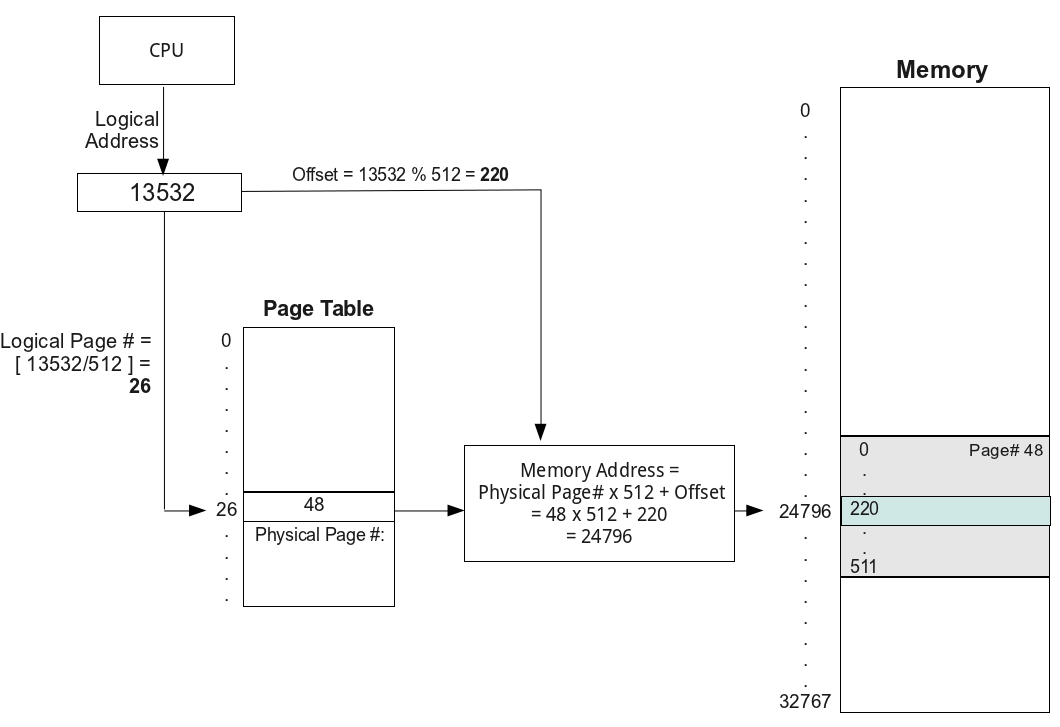
\includegraphics[scale=0.58]{address_translation.png}
	\caption{ \small The logical address generated by the CPU is 13532, so the page number is $\lfloor 13532/512 \rfloor$ = 26 and offset is 13532 mod 512 = 220. The looked up value from the page table is 48. Thus the resultant physical address is 48 $\times$ 512 + 220 = 24796.}
	\label{fig:paging}
\end{figure}




\section{Disk Storage}


\textbf{Block} : It is the basic unit of storage in the disk.\\

The disk can be thought of as consisting of a linear sequence of 512  \textbf{blocks}. The size of each \textbf{block} is equal to that of a page in the memory (512 words). The total disk capacity is 512 $\times$ 512 = 262144 \textbf{words}.\\

Any particular \textbf{block} in the disk is addressed by the corresponding number in the sequence 0 to 511 known as the \textit{block number}.

\begin{figure}[htp!] \small
	\centering
	\begin{tabular}{|c|c|c|c|} 
	\hline
       0 - 511 & 512 - 1023 & ... &   261632 - 262143     \\
       \hline      
      & & & \\ 
      Block 0 & Block 1  & .... & Block 512 \\ 
      & & & \\       
       \hline
       
	\end{tabular}
	\caption{Disk Structure}
	\label{fig:mem_struct}
\end{figure}


\section{Supported Datatypes}

XSM supports 2 different datatypes and their operations, namely \textbf{Strings} and \textbf{Integers}. However in the lowest level data is stored as strings.

\subsection{Strings} Strings are sequence of characters which may include alphabets, numerals and special characters. Every string is terminated with a \textit{null character} ('\textbackslash 0'). Operations that can be performed on strings include lexicographic comparisons.

\subsection{Integers} Integers in XSM can vary from -99999999999999 to +99999999999999. The first character within the word is reserved for the sign. However the integer 0 (zero) would have its sign character as 0 itself. The operations that can be performed on integers include arithmetic operations and comparison operations. A jump can also performed by checking if a register has 0 in it.

 \section{Instructions}
\label{sec:inst}
\subsection{Introduction}

Every instruction in XSM is 2 words long. The instructions provided by the XSM architecture can be classified into privileged and unprivileged instructions. 

\subsection{Classification}

\subsubsection{Unprivileged Instructions}


\begin{enumerate}
\item \texttt{MOV}
\begin{itemize}

\item Register Addressing:\\
\textit{Syntax :} \texttt{MOV Ri, Rj}\\
Copies the contents of the register \texttt{Rj} to \texttt{Ri}.

\item Immediate Addressing:\\
\textit{Syntax :} \texttt{MOV Ri, INTEGER/STRING}
Copies the \texttt{INTEGER/STRING} to the register \texttt{Ri}.


\item Register Indirect Addressing:\\
\textit{Syntax }: \texttt{MOV Ri, [Rj]}\\
Copy contents of memory location pointed by \texttt{Rj} to register \texttt{Ri}.\\
\textit{Syntax :}\texttt{ MOV [Ri], Rj} \\
Copy contents of \texttt{Rj} to the location whose address is in \texttt{Ri}.


\item Direct Addressing:\\
\textit{Syntax :}\texttt{ MOV [LOC], Rj}\\
Copy contents of \texttt{Rj}  to the memory address \texttt{LOC}.\\
\textit{Syntax :} \texttt{MOV Rj, [LOC]}\\
Copy contents of the memory location \texttt{LOC} to the register \texttt{Rj}.

\item Direct Indexed Addressing: \\
\textit{Syntax :}\texttt{ MOV [LOC] Rj, Ri}\\
Copy contents of \texttt{Ri} to the memory address \texttt{LOC} + (value in \texttt{Rj}) \\
\textit{Syntax :}\texttt{ MOV [LOC] Index, Rj}\\
Copy contents of \texttt{Ri} to the memory address \texttt{LOC} + \texttt{Index}. \texttt{Index} must be an integer value. \\
\textit{Syntax :}\texttt{ MOV Ri, [LOC] Rj}\\
Copy contents in the memory address \texttt{LOC} + (value in \texttt{Rj}) to the register \texttt{Ri}\\
\textit{Syntax :}\texttt{ MOV Ri, [LOC] Index}\\
Copy contents of the memory address \texttt{LOC} + \texttt{Index} to the register \texttt{Ri}. \texttt{Index} must be an integer value. \\
\end{itemize}


\item\textbf{ Arithmetic Instructions}
\\
Arithmetic Instructions perform arithmetic operations on registers containing integers. If the register contains a non-integer value, an excpetion is raised (Refer Section \ref{excpetion})
\begin{itemize}
\item \texttt{ADD}, \texttt{SUB}, \texttt{MUL}, \texttt{DIV} and \texttt{MOD}.\\
\textit{General Syntax :} \texttt{OP Ri, Rj}\\
The result of \texttt{Ri} op \texttt{Rj} is stored in \texttt{Ri}. 

\item \texttt{INR\\}
\textit{Syntax :}\texttt{ INR Ri}\\
Increments the value of register \texttt{Ri} by 1.  

\item  \texttt{DCR}\\
\textit{Syntax :} \texttt{DCR Ri}\\
Decrements the value of register \texttt{Ri} by 1. 

\end{itemize}


\item \textbf{Logical Instructions} \\
Logical instructions are used for comparing values in registers. Strings can also be compared according to the lexicographic ordering of ASCII.
\begin{itemize}

\item \texttt{LT}\\
Syntax :\texttt{ LT Ri, Rj}\\
Stores 1 in \texttt{Ri} if the value stored in \texttt{Ri} is less than that in \texttt{Rj}. \texttt{Ri} is set to 0 otherwise. 

\item \texttt{GT}\\
Syntax : \texttt{GT Ri, Rj}\\
Stores 1 in \texttt{Ri} if the value stored in \texttt{Ri} is greater than that in \texttt{Rj}. \texttt{Ri} set to 0 otherwise. 

\item \texttt{EQ}\\
Syntax : \texttt{EQ Ri, Rj}\\
Stores 1 in \texttt{Ri} if the value stored in \texttt{Ri} is equal to that in \texttt{Rj}. Set to 0 otherwise. 

\item \texttt{NE}\\
Syntax : \texttt{NE Ri, Rj}\\
Stores 1 in \texttt{Ri} if the value stored in \texttt{Ri} is not equal to that in \texttt{Rj}. Set to 0 otherwise. 

\item \texttt{GE} \\
Syntax : \texttt{GE Ri, Rj} \\
Stores 1 in \texttt{Ri} if the value stored in \texttt{Ri} is greater than or equal to that in \texttt{Rj}. Set to 0 otherwise. 

\item \texttt{LE}\\
Syntax : \texttt{LE Ri, Rj}\\
Stores 1 in \texttt{Ri} if the value stored in \texttt{Ri} is less than or equal to that in \texttt{Rj}. Set to 0 otherwise. 
\end{itemize}

\item Labels \\
Syntax : \texttt{LABEL \textit{labelname}} \\
Creates a label with a \texttt{\textit{labelname}}  which is a string. Labels are used in branching instruction to specify memory location of target instructions.


\item Branching Instructions\\
Branching is achieved by changing the value of the \texttt{IP} to the address of a specified \texttt{labelname}. 
 
\begin{itemize}
\item \texttt{JZ}\\
Syntax : \texttt{JZ Ri, labelname}\\
Jumps to \texttt{labelname} if the contents of \texttt{Ri} is zero.
\item \texttt{JNZ}\\
Syntax : \texttt{JNZ Ri, labelname}\\
Jumps to \texttt{labelname} if the contents of \texttt{Ri} is not zero.
\item \texttt{JMP}\\
Syntax : \texttt{JMP labelname}\\
Unconditional jump to address specified by \texttt{labelname}\\

\end{itemize}

\item Stack Instructions
\begin{itemize}
\item \texttt{PUSH}\\
Syntax : \texttt{PUSH Ri}\\
Increment \texttt{SP} by 1 and copy contents of \texttt{Ri} to the location pointed to by \texttt{SP}.
\item \texttt{POP}\\
Syntax : \texttt{POP Ri}\\
Copy contents of the location pointed to by \texttt{SP} into \texttt{Ri} and decrement \texttt{SP} by 1.\\
For both these instructions \texttt{Ri} may be any register except \texttt{IP}.
\end{itemize}

\item Subroutine Instructions\\
The \texttt{CALL} instruction copies the address of the next instruction to be fetched on to location \texttt{SP} + 1. It also increments \texttt{SP} by one and transfers control to the \texttt{labelname} specified. The address of the instruction to be fetched is in \texttt{IP + 2} (each instruction is 2 memory words). The \texttt{RET} instruction restores the \texttt{IP} value stored at location pointed by \texttt{SP}, decrements \texttt{SP} by one and continues execution fetching the next instruction pointed to by \texttt{IP}. The subroutine instructions provide a neat mechanism for procedure evocations.
\begin{itemize}
\item \texttt{CALL}\\
Syntax : \texttt{CALL labelname}\\
Increments \texttt{SP} by 1, transfers \texttt{IP}+2 to location pointed to by \texttt{SP} and jumps to \texttt{LABEL}
\item \texttt{RET}\\
Syntax : \texttt{RET}\\
Sets \texttt{IP} to the value pointed to by \texttt{SP} and decrements \texttt{SP}.
\end{itemize}

\item Input/Output Instructions
\begin{itemize}
\item \texttt{IN}\\
Syntax : \texttt{IN Ri}\\
Transfers the contents of the standard input to \texttt{Ri}.
\item \texttt{OUT}\\
Syntax : \texttt{OUT Ri}\\
Transfers the contents of \texttt{Ri} to the standard output.\\
\end{itemize}

\item \texttt{END}\\
Syntax : \texttt{END}\\
This instruction is marks the end of a program.

\item \texttt{INT}\\
Syntax : \texttt{INT n}\\
Generates an interrupt to the kernel with \texttt{n} (1 to 6) as a parameter. It also disables the interrupts. (Read Section \ref{sec:int})
\end{enumerate}


\subsubsection{Privileged Instructions}
There are four privileged instructions. They can only be executed in kernel mode (Refer to \ref{sec:priv_modes}).  These instructions are:
\begin{enumerate}

\item \texttt{IRET}\\
Syntax : \texttt{IRET}\\

Set \texttt{IP} to the value pointed by \texttt{SP} and decrements \texttt{SP} by one. \texttt{IRET} does the same action as \texttt{RET}, but it tells the processor that the interrupt handler has finished. With the execution of the \texttt{IRET} instruction, interrupts are enabled. (Read Section \ref{sec:int})

\item \texttt{LOAD}\\
Syntax : \texttt{LOAD \textit{pagenum} \textit{blocknum}}\\
This instruction loads the block specified by the \texttt{\textit{blocknum}}, from the disk, to the page specified by the \texttt{\textit{pagenum}} in the memory. \texttt{\textit{blocknum}} and \texttt{\textit{pagenum}} should be numbers or registers containing numbers. An excpetion is raised (Refer Section \ref{excpetion}) for invalid arguments or illegal memory access.

\item \texttt{STORE}\\
Syntax : \texttt{STORE \textit{blocknum} \textit{pagenum} }\\ 
This instruction stores the page specified by the \texttt{\textit{pagenum}}, from the memory, to the block specified by the \texttt{\textit{blocknum}}in the disk. \texttt{\textit{blocknum}} and \texttt{\textit{pagenum}} should be numbers or registers containing numbers. An excpetion is raised (Refer Section \ref{excpetion}) for invalid arguments or illegal memory access.

\item \texttt{HALT}\\
Syntax : \texttt{HALT}\\
This instruction causes the machine to halt immediately.
\end{enumerate}

\subsection{Privilege Modes}
\label{sec:priv_modes}
The XSM architecture is interrupt driven and uses a single processor. There are two privilege modes of execution, the user mode and the kernel mode. The privilege mode of execution is determined by the value of IP, i.e. the area in memory where the currently executing code executes. 


\begin{itemize}
\item User mode : Only unprivileged instructions can be executed in this mode. The value of IP cannot be changed in user mode.

\item Kernel mode : Both privileged and unprivileged instructions can be executed in this mode. 

\begin{center}
\begin{tabular}{|c|c|c|}
\hline Page Number & Privilege Space \\ 
\hline 0 & ROM Code \\ 
\hline 1 - 7 & Kernel Space \\ 
\hline 8 - 55 & User Space \\ 
\hline 56 - 63 &  Kernel Space (INT 0 - 7)  \\ 
\hline
\end{tabular} 
\end{center}

\end{itemize}

\section{Interrupts}
\label{sec:int}

\subsection{Introduction}
Interrupts are mechanisms by which the user code interrupts the execution of the processor and passes control to the kernel to accomplish low level functionalities like disk access, multiprogramming etc. There are 8 interrupts (numbered from 0 to 7) supported by the XSM architecture. The interrupt 0 is for hardware interrupts, the interrupts (1 to 7) are software interrupts.\\



\subsection{Hardware Interrupts }
Hardware Interrupts are generated by the machine, usually at set timer intervals. These interrupts cannot be invoked from the user/kernel mode.\\

\textbf{Interrupt 0:} \\
It transfers control of execution, i.e. changes the value of IP to \textit{page number} 56 (address = 28672). This is the timer interrupt which interrupts the processor. Generally it is supposed to contain the code for the scheduler of the operating system, which schedules the CPU time among the various active processes.

\subsection{Software Interrupts }
Software Interrupts interrupts are unprivileged and can be called from user mode.
\subsubsection{The \texttt{INT} instruction}
The instruction used to generate a software interrupt is \texttt{INT}.\\
Syntax : \texttt{INT n}\\
The \texttt{INT} instruction passes control to the Interrupt Service Routine (ISR) for this interrupt located at the physical address computed using the value n.

Address computation is done as follows. The physical address of the ISR corresponding to interrupt number n is given by: 
\begin{verbatim}
Physical Address = (56 + n) x Page Size
\end{verbatim}
Note that the interrupts are disabled once this instruction is executed as interrupts cannot be executed in kernel mode.

\begin{itemize}

\item \texttt{INT 1}  \\It transfers control of execution to \textit{page number} 57 (address = 29184)
\item \texttt{INT 2}  \\It transfers control of execution to \textit{page number} 58 (address = 29696)  
\item \texttt{INT 3}  \\It transfers control of execution to \textit{page number} 59 (address = 30208)
\item \texttt{INT 4}  \\It transfers control of execution to \textit{page number}  60 (address = 30720) 
\item \texttt{INT 5}  \\It transfers control of execution to \textit{page number} 61 (address = 31232)
\item \texttt{INT 6}  \\It transfers control of execution to \textit{page number} 62 (address = 31744)
\item \texttt{INT 7}  \\It transfers control of execution to \textit{page number} 63 (address = 32256).\
 
\end{itemize}

\section{Exceptions}
\label{excpetion}
Exceptions are anomalous situations which changes the normal flow of execution. Exceptions usually requires special processing. It is generated when the following events occur:

\begin{enumerate}
\item Illegal memory access : occurs when any address generated by the process \textbf{does not} lie in the range \textbf{[0, 2047]}.
\item Arithmetic exception : occurs when divisor is 0.
\item Illegal operands : occurs when operands contain invalid data corresponding to the instruction. 
\item Illegal instruction : occurs when an attempt is made to execute an instruction not belonging to the instruction set and also when the operands to the instruction is not legal. Eg: \texttt{MOV 4 R0}, \texttt{MOV IP 4} when executed in user mode. These instructions are considered illegal.
\item Stack overflow and stack underflow : Stack overflow occurs when the value in the \texttt{SP} register exceeds \textbf{2047} and stack underflow occurs when the value falls below \textbf{1536}.
\end{enumerate}


\end{document}